\documentclass{llncs}

\usepackage{amssymb}
\setcounter{tocdepth}{3}
\usepackage{graphicx}
\usepackage[ruled]{algorithm2e}
%\usepackage[lined,boxed,commentsnumbered]{algorithm2e}
\usepackage{amssymb}
\usepackage{amsmath,graphicx,color,doi}
\usepackage{algorithm2e}
%\usepackage{algorithmic}	
\usepackage{multirow}
\usepackage{subfigure}
\usepackage{cite}


\newcommand{\gi}[1]{{\textcolor{red}{[\small \textbf{Giacomo}: #1]}}}
\newcommand{\ad}[1]{{\textcolor{red}{[\small \textbf{Adriano}: #1]}}}
\newcommand{\cl}[1]{{\textcolor{red}{[\small \textbf{Claudio}: #1]}}}

\begin{document}
\title{Tampering detection for low-power smart cameras}

\author{Adriano Gaibotti\inst{1}\inst{2} \and Claudio Marchisio\inst{2} \and Alexandro Sentinelli\inst{2} \and Giacomo Boracchi\inst{1}}

\institute{ 
	Politecnico di Milano, Dipartimento di Elettronica, Informazione e Bioingegneria (DEIB), Via Ponzio 34/5, 20133, Milano (MI), Italy\\
	\email{adriano.gaibotti@mail.polimi.it, giacomo.boracchi@polimi.it}
	\and
	STMicroelectronics, Advanced System Technology, Via Camillo Olivetti 2, 20864, Agrate Brianza (MB), Italy\\
	\email{\{adriano.gaibotti, claudio.marchisio, alexandro.sentinelli\}@st.com}
}
\maketitle

\begin{abstract}
One of the most critical issues in smart cameras, used as nodes in wireless multimedia sensor networks (WMSN), is the automatic detection of events that could compromise the correct acquisition of the scene, such as the presence of water on the camera lens, or the displacement of the device, or tampering events. 
In general, techniques used to identify these type of events are called tampering detection algorithms.
We introduce a solution for the tampering detection issue which can be used for low-power and embedded smart cameras, in which the acquisition is done with low frame rate, such as one frame every minute.
The solution consists in a segmentation of the acquired scene in adaptive regions, and monitoring some features in each region, in order to find a change in their behavior that could be associated to a tampering event.
Experiments show that our solution increase the performances with respect to monitoring the whole scene, with low computational complexity.
\keywords{tampering, defocus, displacement, segmentation, gradient}
\end{abstract}



\section{Introduction}\label{sec:introduction}

\gi{Adriano: metti un paio di foto per spiegare il problema che consideriamo.}



\begin{figure}
\centering
\subfigure[]{\label{fig:neve} 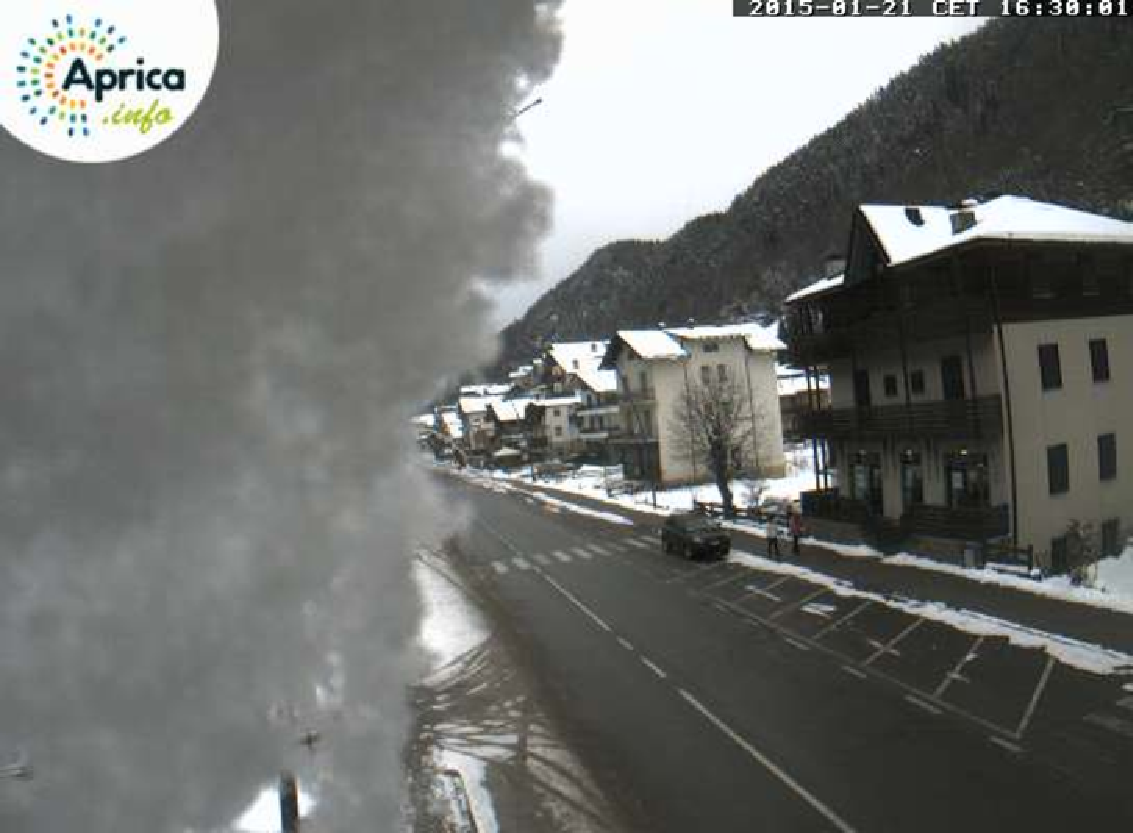
\includegraphics[width=0.4\linewidth]{Immagini/neve}}
\subfigure[]{\label{fig:pioggia} 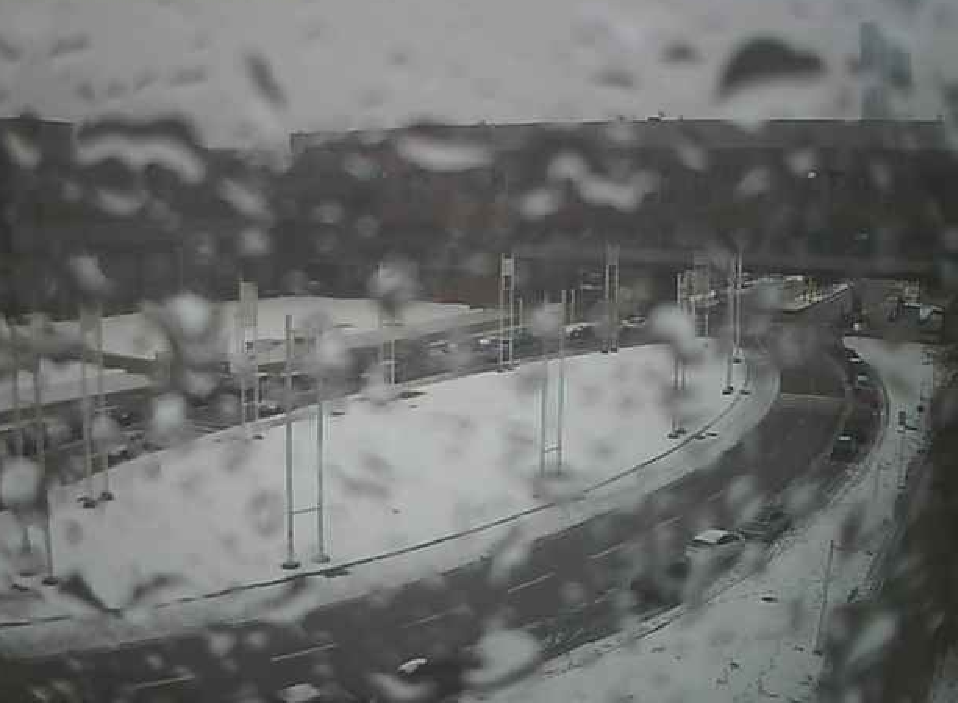
\includegraphics[width=0.4\linewidth]{Immagini/pioggia}}
\caption[Tampering examples]{Examples of tampering events due to atmospheric phenomena. In Figure \ref{fig:neve} there is an occlusion due to some snow on the camera lens, while in Figure \ref{fig:pioggia} there is a blur due to rain drops on the camera lens.}
\label{fig:tampering}
\end{figure}


Random Toughs:
\begin{itemize}
\item Smart cameras, low-power monitoring of scene. Description of the application scenario. Low frame rate.
\item Cameras organized in a multimedia network, continuous acquisition and streaming is not feasible
\item The problem of false alarms, radio module activation
\item Other tampering attacks like obfuscation (??) which might be due to environmental phenomena such as rain, fog and mist over the camera lenses have to be detected by image analysis methods
\item Displacement can be perceived by MEMS as well but these device alone are prone to false alarms. Visual inspection is necessary to reduce false alarms
\item constrained environment: algorithms have to operate with a low computational complexity and memory requirement
\end{itemize}

 
\section{Related Works}\label{sec:relWorks}

\gi{Adriano: metti tutte le reference, ciascuna con un commento di una frase per dire che fa ed una frase (o mezza) per dire i problemi che ha (con particolare riferimento all'ambito low-power) Poi le aggiustiamo in maniera organica}

\cite{aksay2007camera}: uses background subtraction methods in order to identify defocus and occlusions, doing a comparison in the wavelet domain for defocus detection and histogram comparison  for occlusion detection. Displacement is not treated.

\cite{saglam2009real}:  uses background subtraction methods in order to identify defocus, occlusions, and displacements. Comparison in the Fourier domain for defocus detection, histogram comparison for occlusion detection, comparison between current background and delayed background for displacement detection.

\cite{alippi2010detecting}: CUSUM CDT on gradient energy content in order to detect blur in frames 

\cite{gil2007automatic}:  uses background subtraction methods in order to identify defocus, occlusions, and displacements. Comparison of edges pixels count for defocus detection, entropy comparison for occlusion detection, block matching algorithm for displacement detection.

\cite{ribnick2006real}: comparison between frames belonging to a buffer in order to find high values of dissimilarity, associated to tampering.

\cite{kryjak2012fpga}: implementation in a FPGA of a solution based on background modeling, histograms comparisons, edges comparisons.

\cite{harasse2004automated}: tampering detection inside a moving vehicle; uses background subtraction methods in order to identify defocus, occlusions, and displacements. Comparison of edges pixels count for defocus detection, entropy comparison for occlusion detection, block matching algorithm for displacement detection.

\cite{tsesmelis2013tamper}: monitoring of the number of key points extracted by SURF in order to detect defocus events, partition in blocks and HOG descriptors matching for each block in order to detect occlusions. These types of solutions requires a lot of computations

\section{Problem Formulation}\label{sec:probForm}

\gi{Adriano: metti le formule di quello della tesi circa displacemente e out of focus. Poi condensiamo il tutto}


\begin{equation}
\label{eq:blur_single}
z(x)=\mathcal{D}[y](x) = \mathcal{B}[y](x) + \eta(x), \qquad x \in \mathcal{X}
\end{equation}


\begin{equation}
\label{eq:blur}
\mathcal{B}[y](x) = \int_{\mathcal{X}}y(s)h(x,s)ds,
\end{equation}


\begin{equation}
\label{eq:blur_convolution}
\mathcal{B}[y](x) = \int_{\mathcal{X}}y(s)h(s-x)ds,
\end{equation}

\begin{equation}
\label{eq:blur_multi}
z_t(x)=\mathcal{D}_t[y_t](x) = \mathcal{B}_t[y_t](x) + \eta(x), \qquad x \in \mathcal{X}.
\end{equation}

\begin{equation}
\label{eq:displacement}
z_t(x)  = \left\{ \begin{array}{rcl}
y_t(x) + \eta(x) & \mbox{per} & t < T^* \\
w_t(x) + \eta(x) & \mbox{per} & t \geqslant T^*
\end{array}\right. ,
\end{equation}


Per $t<T^*$ abbiamo che i frame vengono acquisiti in condizioni di funzionamento normale:
\[ z_t(x)=y_t(x) + \eta(x), \forall x \in \mathcal{X} \mbox{, per } t=1,\dots , T^*-1. \] 
All'istante di tempo $t = T^*$ avviene un evento di tampering, il quale compromette i frame per $t\geq T^*$.  
In particolare, nel caso di una sfocatura avremo
\[ z_t = \mathcal{B}_t[y_t](x) + \eta(x), \forall x \in \mathcal{X} \mbox{, per } t \geq T^*,\]
mentre nel caso di uno spostamento della camera avremo
\[ z_t = w_t(x) + \eta(x), \forall x \in \mathcal{X} \mbox{, per } t \geq T^*. \]



\section{Proposed Solution}\label{sec:propSol}




\subsection{Scene Segmentation}\label{subsec:Segmentation}
Consideriamo la sequenza $\{z_t\}$ di frame acquisiti dalla camera, con $t=1,\dots,T_{c}$.
Per ciascun pixel $x\in\mathcal{X}$ calcoliamo un vettore $\textbf{d}(x)$ di $5$ elementi
\begin{equation}
\label{eq:featureVector}
\textbf{d}(x)=\left[r(x);c(x);\mu_{\nabla}(x);\sigma_{\nabla}(x);\bar{z}(x)\right], \textbf{d}(x) \in \mathbb{R}^5
\end{equation}
dove:
\begin{itemize}
	\item $r(x)$ rappresenta il numero di riga del pixel $x$.
	\item $c(x)$ rappresenta il numero di colonna del pixel $x$.
	\item $\mu_{\nabla}(x)$ rappresenta il valore del gradiente nel pixel $x$ mediato nel tempo:
	\begin{equation}
	\label{eq:segmentazioneGrad}
	\mu_{\nabla}(x) = \frac{\sum_{t=1}^{T_c}(\|\nabla z_t\|_2^2 \circledast f)(x)}{T_c},
	\end{equation}
	dove abbiamo indicato con $\|\nabla z_t\|_2^2$ la norma del gradiente per l'immagine $z_t$, definita in \eqref{eq:normaGradiente}, e con $f$ il filtro gaussiano discreto derivato dal campionamento di \eqref{eq:gaussian}.
	\item $\sigma_{\nabla}(x)$ rappresenta la deviazione standard nel tempo del gradiente nel pixel $x$:
	\begin{equation}
	\label{eq:segmentazioneVar}
	\sigma_{\nabla}(x)=\sqrt{\frac{1}{T_c - 1}\sum_{t=1}^{T_c}\left(\left(\|\nabla z_t\|_2^2 \circledast f\right)(x)-\mu_{\nabla}(x)\right)^2}.
	\end{equation}
	\item $\bar{z}(x)$ rappresenta il valore della luma del pixel $x$ mediato nel tempo:
	\begin{equation}
	\label{eq:segmentazioneLuma}
	\bar{z}(x)=\frac{\sum_{t=1}^{T_c}( z_t \circledast f)(x)}{T_c}.
	\end{equation}
\end{itemize}
\subsection{Indicators}\label{subsec:Indicators}
\gi{Adriano: mettere formule degli indicatori e anche del frame difference qua}

\begin{equation}
\label{eq:gradientRegions}
\begin{array}{ccc}
g^k(t)&  = & \mathcal{G}^k[z_t] = \frac{\sum_{\mathcal{R}_k}\| \nabla z_t(x) \| _2^2 }{|{\mathcal{R}_k}|}\\
\partial g^k(t) & =& g^k(t)-g^k(t-1) 
\end{array},
\end{equation}

In particolare, per il calcolo delle derivate orizzontali  abbiamo utilizzato il seguente filtro $f_h$:
\[f_h = f \circledast \left[ \begin{array}{rcl}
1 & 0 & -1
\end{array}\right], \] 
mentre per il calcolo delle derivate verticali abbiamo utilizzato il seguente filtro $f_v$:
\[f_v = f \circledast \left[ \begin{array}{r}
1 \\ 0 \\ -1
\end{array}\right], \]
dove abbiamo indicato con $\circledast$ l'operatore di convoluzione.
Il filtro $f$, invece, \`e ottenuto tramite un campionamento della \textit{funzione gaussiana} $h$, con media $0$ e deviazione standard $\sigma$
\begin{equation}
\label{eq:gaussian}
h(i,j)=\frac{1}{2\pi\sigma^2}\exp\left(-\frac{i^2+j^2}{2\sigma^2}\right),
\end{equation}
e ponendo il valore massimo di questa funzione nel centro del filtro.
Con questi filtri \`e possibile calcolare la \textit{norma del gradiente} nel seguente modo:
\begin{equation}
\label{eq:normaGradiente}
\| \nabla z_t(x) \|_2^2=\left(z_t \circledast f_h\right)(x)^2 + \left(z_t \circledast f_v\right)(x)^2.
\end{equation}
Una volta calcolata la norma del gradiente \`e possibile farne la media come specificato in \eqref{eq:energyGradient}.
Il risultato finale \`e un indicatore \textit{scalare} per ciascun frame acquisito, che pu\`o essere monitorato per individuare eventi di sfocature. 
In particolare ci aspettiamo che l'evento di sfocatura provochi un abbattimento del valore di $g$.



\begin{equation}
\label{eq:lumaRegions}
\begin{array}{ccc}
l^k(t)&  = & \mathcal{L}^k[z_t] = \frac{\sum_{\mathcal{R}_k} z_t(x) }{|{\mathcal{R}_k}|}\\
\partial l^k(t) & =& l^k(t)-l^k(t-1) 
\end{array},
\end{equation}


\begin{equation}
\label{eq:energyLuma}
l(t) = \mathcal{L}[z_t] =\frac{\sum_{\mathcal{X}} z_t(x) }{|\mathcal{X}|} ,
\end{equation}  


\begin{equation}
\label{eq:gradientDetr}
\frac{\partial g}{\partial t}(t) = g(t) - g(t-1),
\end{equation}


\begin{equation}
\label{eq:lumaDetr}
\frac{\partial l}{\partial t}(t) = l(t) - l(t-1).
\end{equation}


\subsection{Outlier Detection}\label{subsec:MonitoringScheme}



\begin{equation}
\label{eq:soglieGradiente}
\begin{array}{lcl}
\Gamma_{min}^k & = & \hat{\mu}_g^k -\gamma \hat{\sigma}_g^k\\
\Gamma_{max}^k & = & \hat{\mu}_g^k + \gamma \hat{\sigma}_g^k
\end{array},
\end{equation}
dove $\hat{\mu}_g^k$ indica il valore medio delle osservazioni del training set
\begin{equation}
\hat{\mu}_g^k = \frac{\sum_{\tau = 1}^{T_{o}} \frac{\partial g^k}{\partial t}(\tau)}{T_{o}}, \nonumber
\end{equation}
$\hat{\sigma}_g^k$ indica la deviazione standard delle osservazioni del training set
\begin{equation}
\hat{\sigma}_g^k  = \sqrt{\frac{1}{T_{o}-1}\sum_{\tau=1}^{T_{o}}\left(\frac{\partial g^k}{\partial t}(\tau) - \hat{\mu}_g^k(\tau)\right)^2} \nonumber
\end{equation}
e $\gamma>1$ \`e un parametro moltiplicativo ottenuto sperimentalmente.\\

\begin{equation}
\label{eq:soglieLuma}
\begin{array}{rcl}
\Gamma_{min}^k & = & \hat{\mu}_l^k -\gamma \hat{\sigma}_l^k\\
\Gamma_{max}^k & = & \hat{\mu}_l^k + \gamma \hat{\sigma}_l^k
\end{array},
\end{equation}
dove $\hat{\mu}_l^k$ indica il valore medio delle osservazioni del training set
\begin{equation}
\hat{\mu}_l^k = \frac{\sum_{\tau = 1}^{T_{o}} \frac{\partial l^k}{\partial t}(\tau)}{T_{o}}, \nonumber
\end{equation}
$\hat{\sigma}_l^k$ indica la deviazione standard delle osservazioni del training set
\begin{equation}
\hat{\sigma}_l^k  = \sqrt{\frac{1}{T_{o}-1}\sum_{\tau=1}^{T_{o}}\left(\frac{\partial l^k}{\partial t}(\tau) - \hat{\mu}_l^k(\tau)\right)^2} \nonumber
\end{equation}
e $\gamma>1$ \`e un parametro moltiplicativo ottenuto sperimentalmente.\\





\subsection{Algorithm Summary}\label{subsec:AlgorithmSummary}



%\begin{algorithm}[tp]
%	% \SetAlgoNoLine
%	\LinesNumbered
%	\SetAlgoNlRelativeSize{0}
%	\SetNlSty{small}{}{.}
%	\textbf{Configuration}:\\
%	\lnl{DEF-Tr0} Extract regions $\{R_k\}, k=1,\dots,K$  \\
%	\lnl{DEF-Tr1} \For{$t=1,\dots,T_{o}$}
%	{	\lnl{DEF-Tr2} Acquire frame $z_t$ \\
%		\lnl{DEF-Tr2a} \For{$k=1,\dots,K$}{
%			\lnl{DEF-Tr3a} Compute $g^k(t)$, $\frac{\partial g^k}{\partial t}(t)$ for the region $R_k$\\
%		}
%		\lnl{DEF-Tr3} Compute $g(t)$, $\frac{\partial g}{\partial t}(t)$ \\
%	}
%	\lnl{DEF-Tr6a} \For{$k=1,\dots,K$}{
%		\lnl{DEF-Tr7a} Define thresholds $\Gamma_{min}^k$ and $\Gamma_{max}^k$\\
%	}
%	\lnl{DEF-Tr5} Define CDT parameters on $g(t)$ variance\\
%	\textbf{Operational phase}:\\
%	\lnl{DEF-Test1} \For{$t=T_{o},\dots,\infty$}{
%		\lnl{DEF-Test2} Acquire frame $z_t$ \\
%		\lnl{DEF-Tr3b} Compute $g(t)$, $\frac{\partial g}{\partial t}(t)$ \\
%		\lnl{DEF-Test2a} $n=0$\\
%		\lnl{DEF-Test4a} \For{$k=1,\dots,K$}{
%			\lnl{DEF-Test5a} Compute $g^k(t)$, $\frac{\partial g^k}{\partial t}(t)$ for the region $R_k$\\
%			\lnl{DEF-Test6a} \If{$\frac{\partial g^k}{\partial t}(t) < \Gamma_{min}^k \vee \frac{\partial g^k}{\partial t}(t) > \Gamma_{max}^k $}{
%				\lnl{DEF-Test7a} $n=n+1$\\
%			}
%		}
%		\lnl{DEF-Test81} \If{$n \geq K-1$}{
%			\lnl{DEF-Test91} $z_t$ is a defocused frame\\
%		}
%		\lnl{DEF-Test8} \If{CDT detect a change on $g(t)$ variance}{
%			\lnl{DEF-Test9} $z_t$ is a defocused frame\\
%		}
%	}   
%	\caption{Blur detection algorithm}
%	\label{alg:DEFOCUS}
%\end{algorithm}

\begin{algorithm}[tp]
	% \SetAlgoNoLine
	\LinesNumbered
	\SetAlgoNlRelativeSize{0}
	\SetNlSty{small}{}{.}
	\textbf{Input}: $\gamma$, $T_{o}$, $\{\mathcal{R}_k\}, k=1,\dots,K$ \\
	\textbf{Configuration}:\\
%	\lnl{DISPL-Tr1} Extract regions $\{\mathcal{R}_k\}, k=1,\dots,K$  \\
	\lnl{DISPL-Tr2} \For{$t=1,\dots,T_{o}$}
	{	\lnl{DISPL-Tr3} Get frame $z_t$ \\
		\lnl{DISPL-Tr4} \For{$k=1,\dots,K$}{
			\lnl{DISPL-Tr5} Compute $l^k(t)$, $\partial l^k(t)$ for the region $\mathcal{R}_k$\\
		}
	}
	\lnl{DISPL-Tr6} \For{$k=1,\dots,K$}{
		\lnl{DISPL-Tr7} Compute $\sigma_l^k$\\
	}
	\textbf{Operational phase}:\\
	\lnl{DISPL-Test1} \For{$t=T_{o},\dots,\infty$}{
		\lnl{DISPL-Test2} Get frame $z_t$ \\
		\lnl{DISPL-Test3} $n_l = 0$ \\
		\lnl{DISPL-Test4} \For{$k=1,\dots,K$}{
			\lnl{DISPL-Test5} Compute $l^k(t)$, $\partial l^k(t)$ for the region $\mathcal{R}_k$\\
			\lnl{DISPL-Test6} \If{$\partial l^k(t) < -\gamma \sigma_l^k \vee \partial l^k(t) > \gamma \sigma_l^k $}{
				\lnl{DISPL-Test7} $n_l=n_l+1$\\
			}
		}
		\lnl{DISPL-Test8} \If{$n_l\geq K-1$}{
			\lnl{DISPL-Test9} $z_t$ is a tampered frame\\
		}
	}   
	\caption{Tampering detection algorithm}
	\label{alg:DISPL}
\end{algorithm}
\gi{Adriano: inserisci qui l'algoritmo e traducilo in inglese. Se riusciamo lo spostiamo prima di tutte le sottosezioni}

\section{Experiments}\label{sec:experiments}
\begin{figure}
\centering
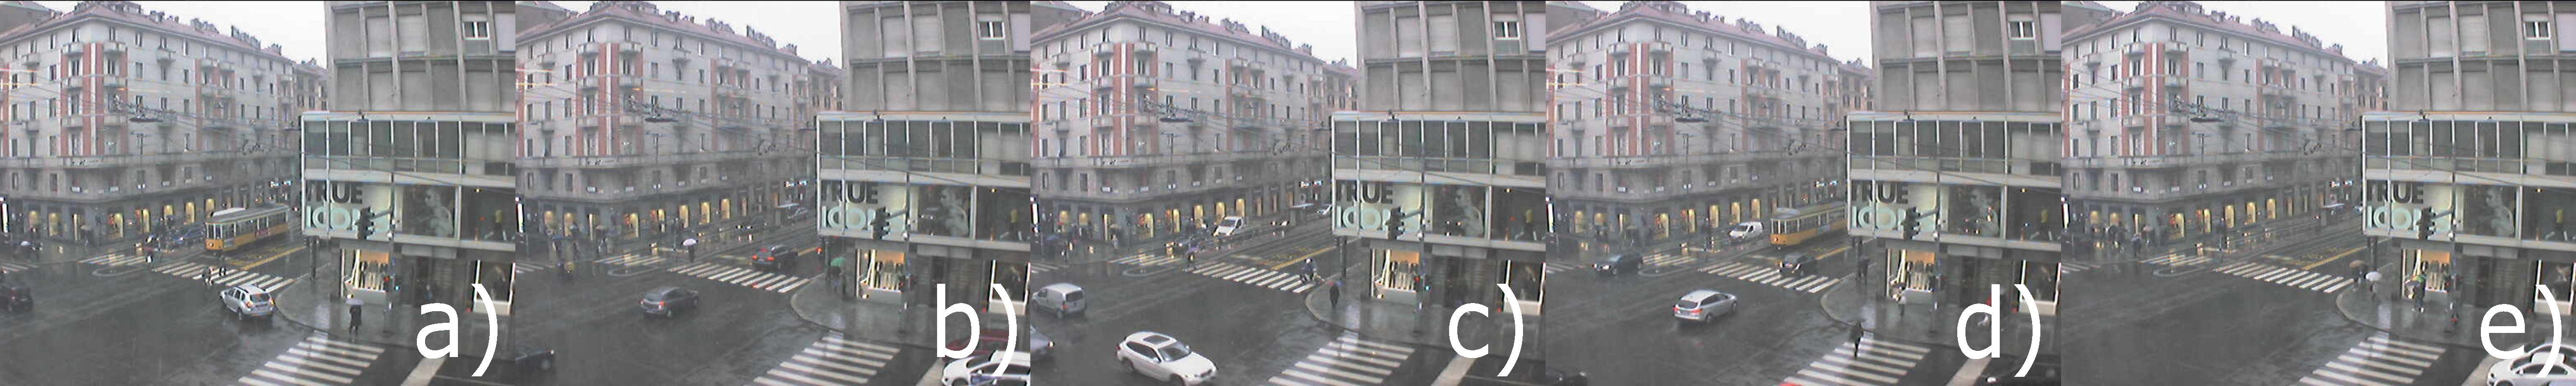
\includegraphics[width=1\linewidth]{Immagini/buenosAires}
\caption{}
\label{fig:buenosAires}
\end{figure}
\begin{figure}
\centering
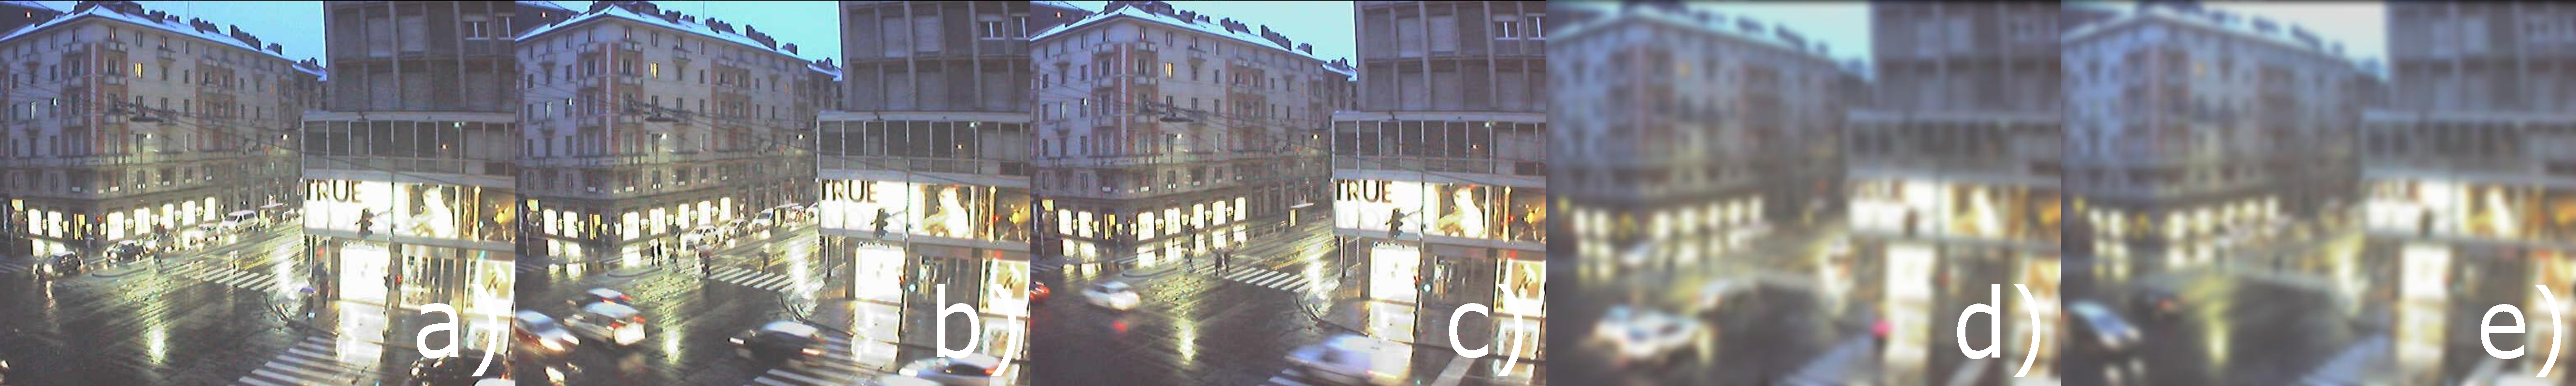
\includegraphics[width=1\linewidth]{Immagini/buenosAiresDef}
\caption{}
\label{fig:buenosAiresDef}
\end{figure}
\begin{figure}
\centering
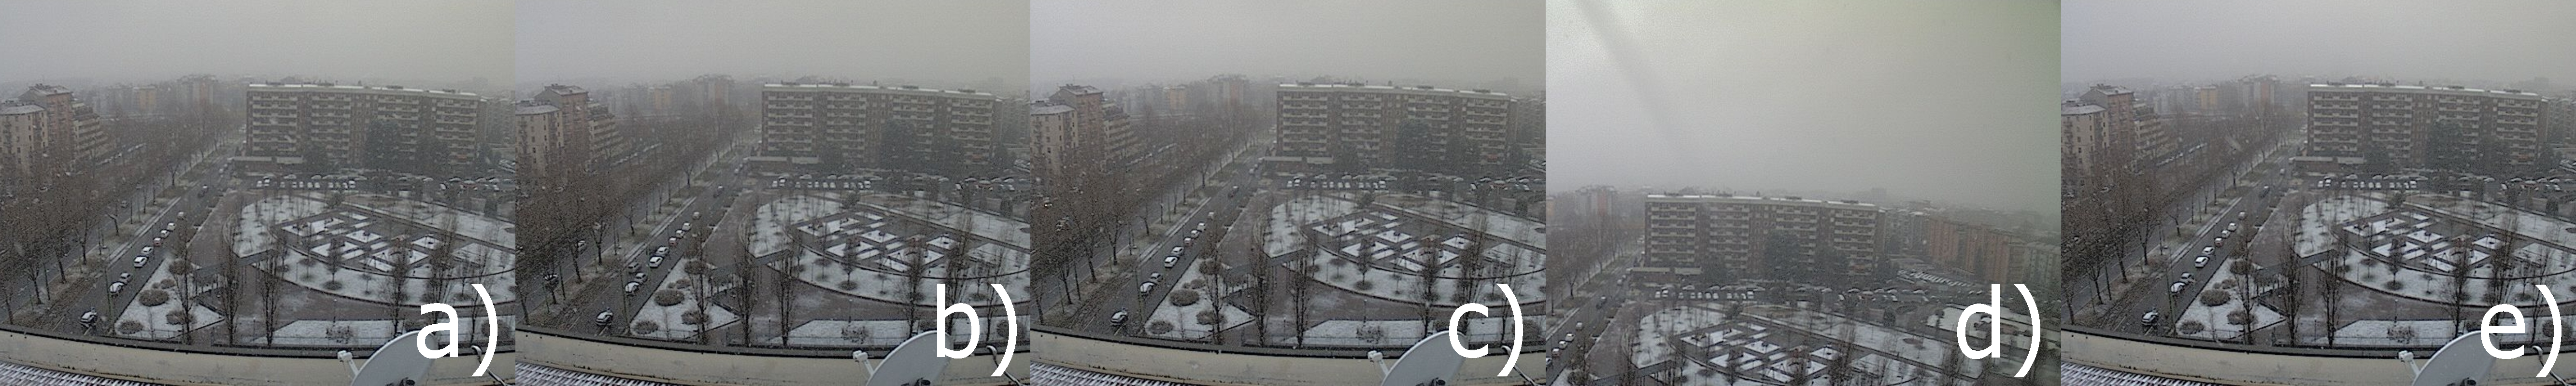
\includegraphics[width=1\linewidth]{Immagini/fulvioTestiDispl}
\caption{}
\label{fig:fulvioTestiDispl}
\end{figure}

\subsection{Dataset Description}\label{subsec:Dataset}
\gi{Adriano: Prova a mettere qua le info}
The proposed method have been tested on a dataset of frame sequences in which there were tampering events.
A part of this dataset was taken using a Raspberry Pi with its camera module, and the tampering was introduced by moving the device or putting water on the camera.
The other part of this dataset is made of frame sequences taken from web-cams available on the Internet. 
In these sequences there were a few events of displacements or defocus, but to have a larger set of tampering events we
\subsection{Alternative Approaches}\label{subsec:AlternativeApproaches}
\begin{itemize}
\item Full
\item Adaptive Region
\item Voronoi Regions
\end{itemize}

\subsection{Performance Assessment}
\gi{Adriano: Dire come vengono calcolate le ROC curves TPR e FPR, le cifre di merito insomma, spiegando bene che parametro varia}

\gi{Adriano: metti entrambe le ROC curves, affiancate e per bene ed alcuni esempi di sequenze}

\begin{figure}
	\centering
	\subfigure[]{\label{fig:ROCdisplZOOM} 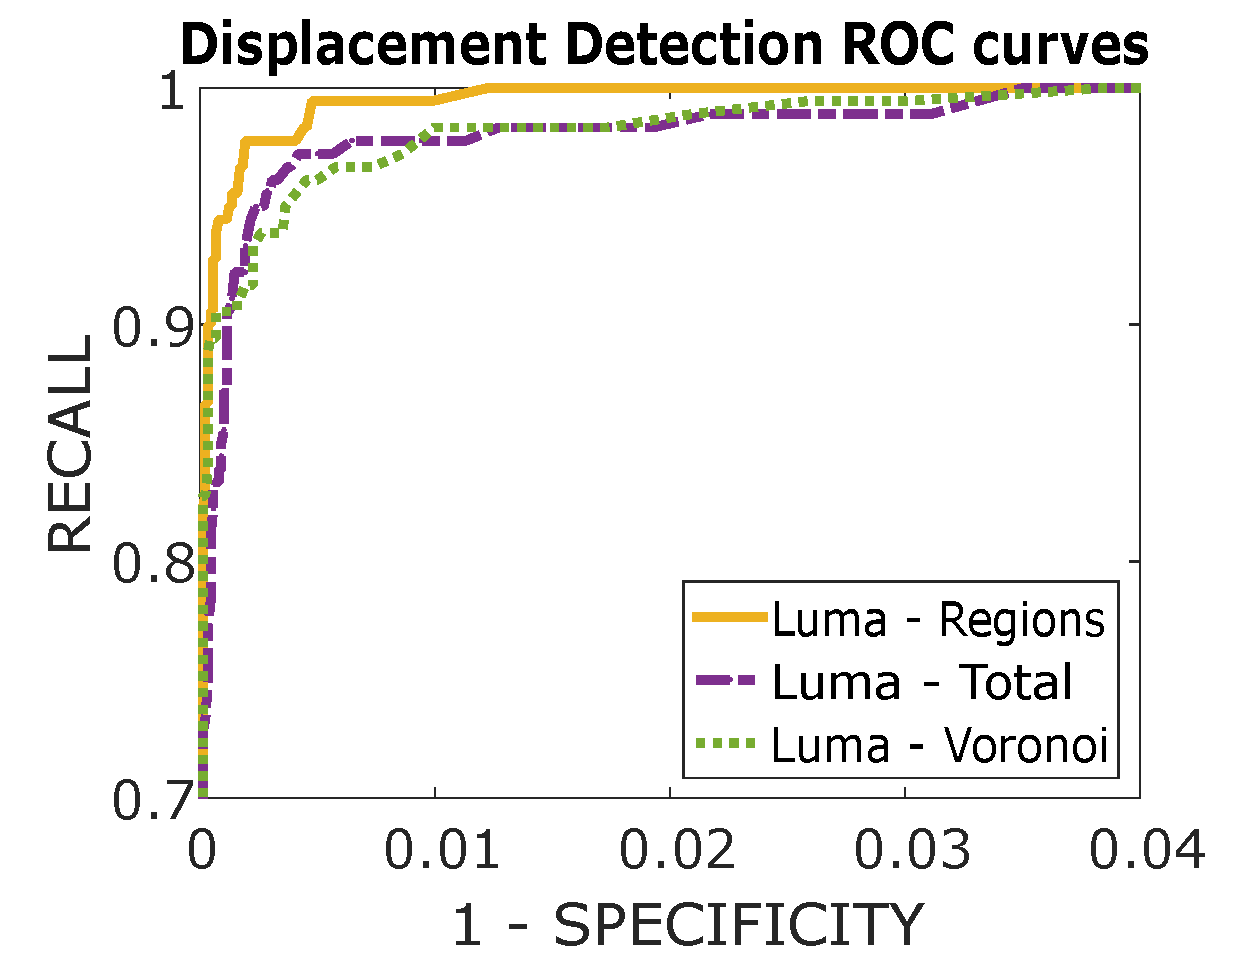
\includegraphics[width=0.45\linewidth]{Immagini/ROCdisplacementZOOM.pdf}}
%	\subfigure[]{\label{fig:ROCdefocus} 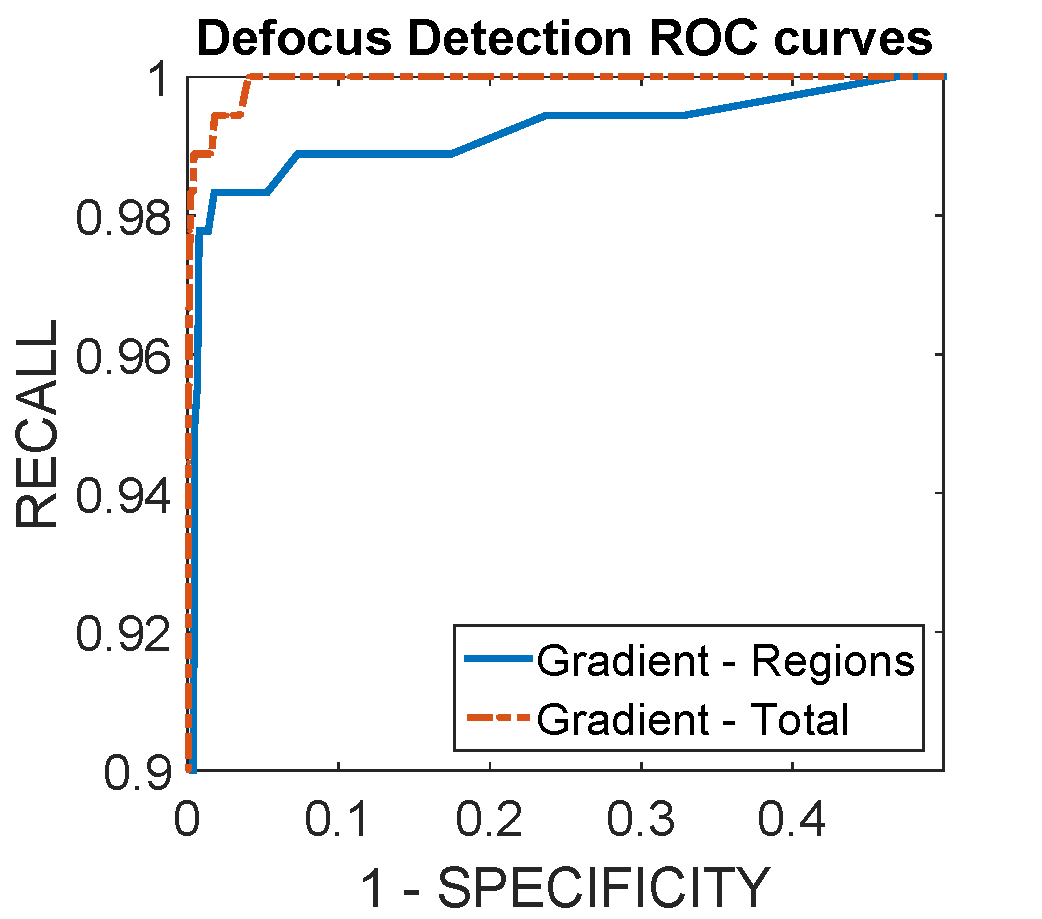
\includegraphics[width=0.45\linewidth]{Immagini/ROCdefocus.pdf}}
	\subfigure[]{\label{fig:ROCdefocusZOOM} 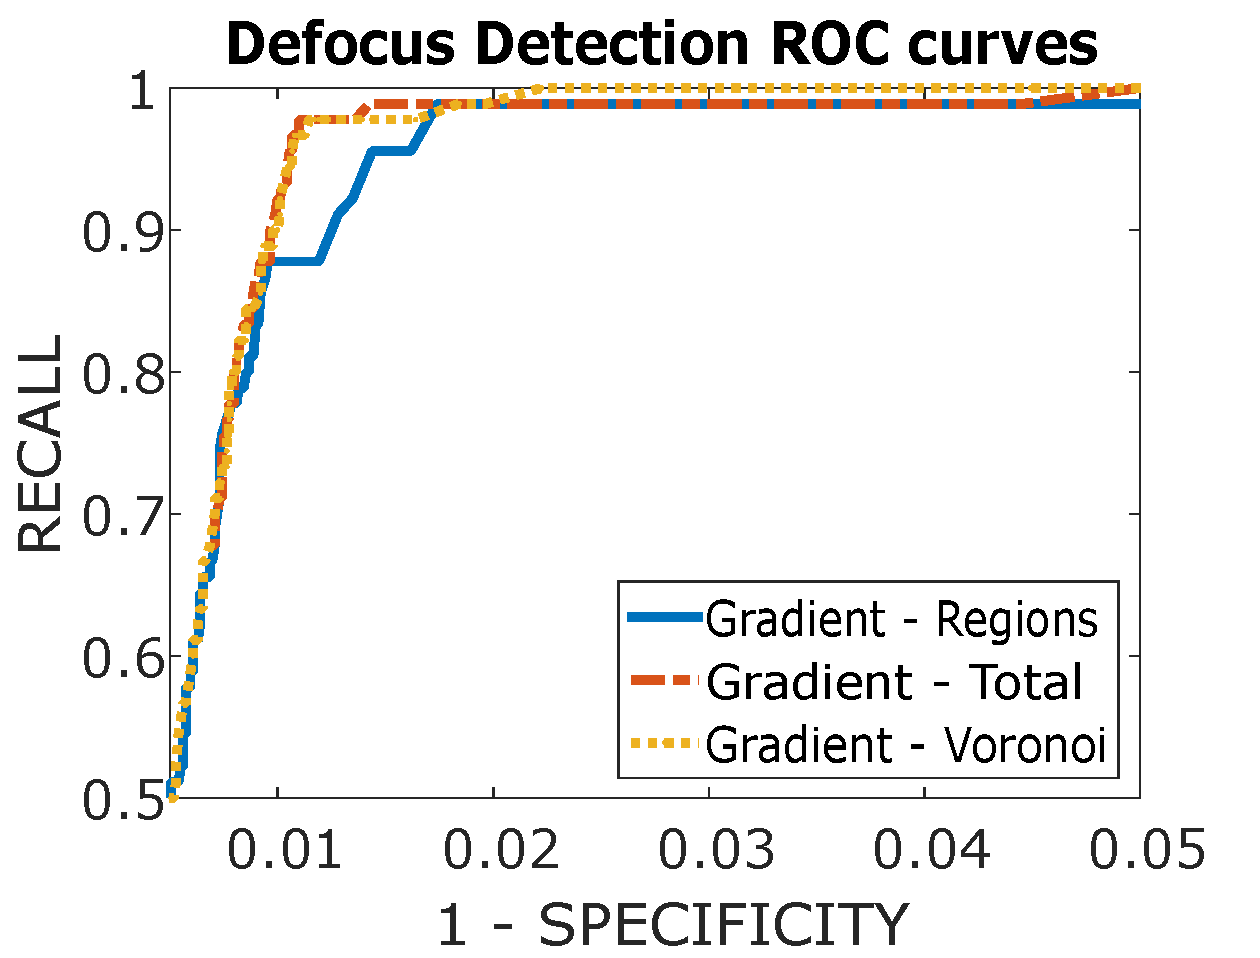
\includegraphics[width=0.45\linewidth]{Immagini/ROCdefocusZOOM.pdf}}
%	\subfigure[]{\label{fig:ROCdispl} 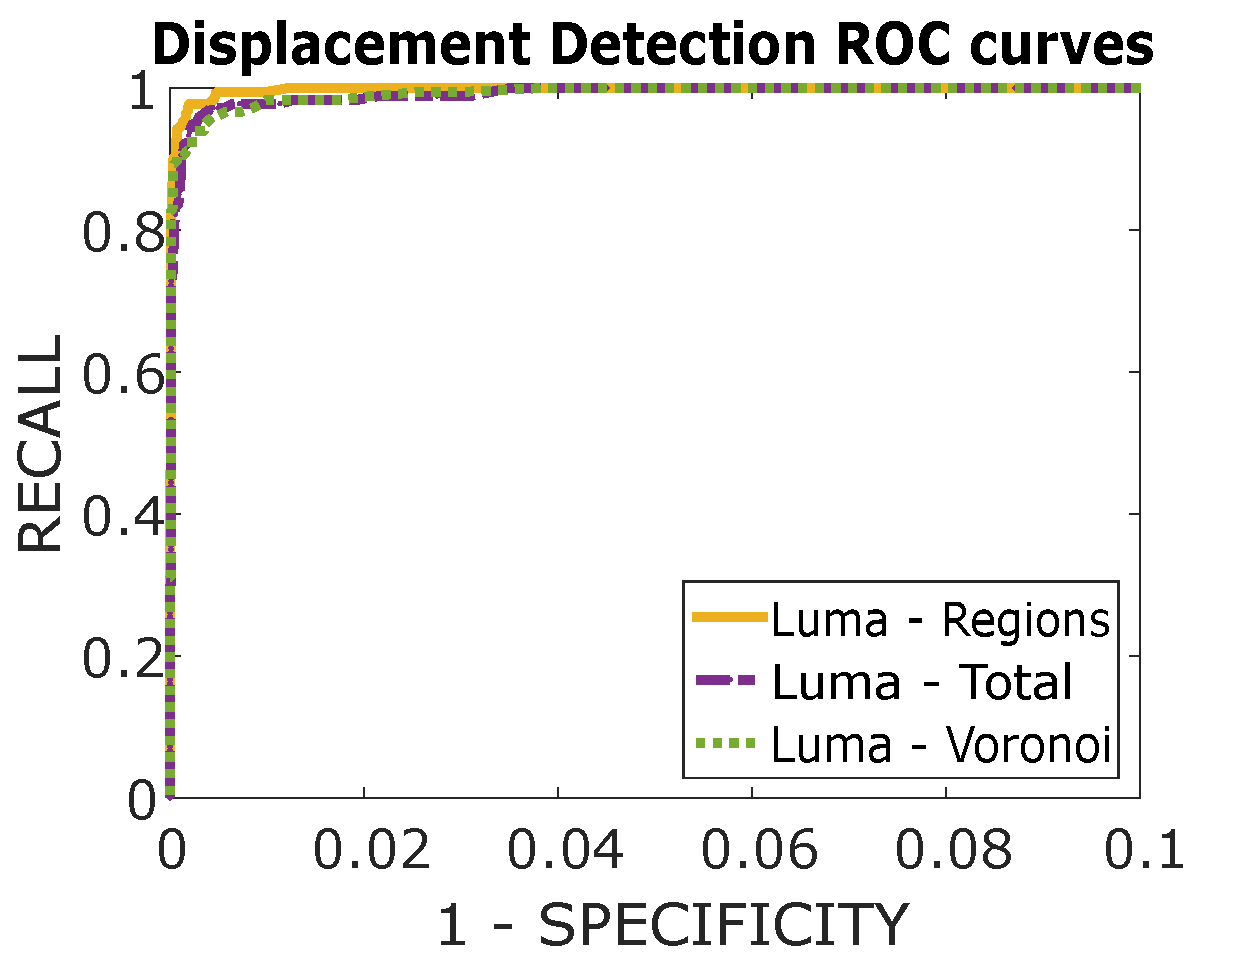
\includegraphics[width=0.45\linewidth]{Immagini/ROCdisplacement.pdf}}
	\caption[Tampering examples]{Examples of tampering events due to atmospheric phenomena. In Figure \ref{fig:neve} there is an occlusion due to some snow on the camera lens, while in Figure \ref{fig:pioggia} there is a blur due to rain drops on the camera lens.}
	\label{fig:ROC}
\end{figure}


%\begin{figure}
%\centering
%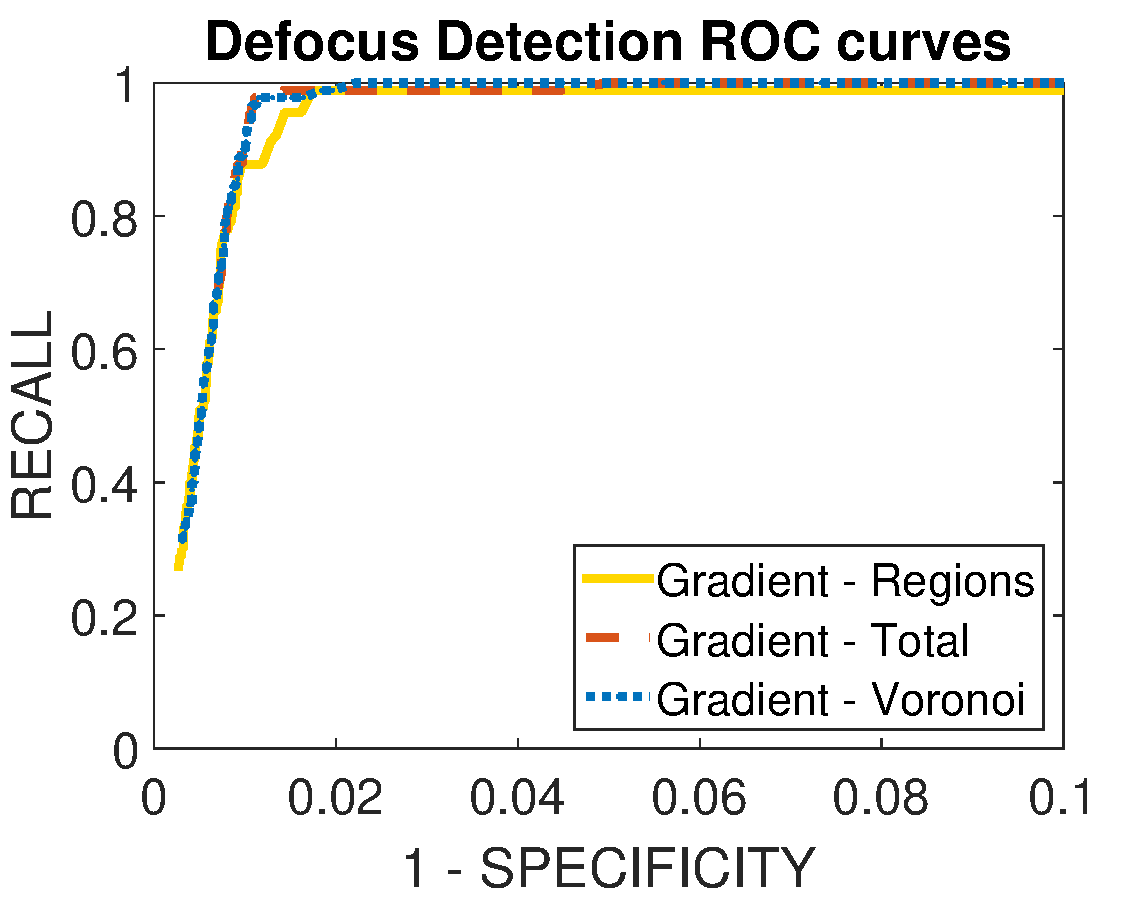
\includegraphics[width=0.7\linewidth]{Immagini/ROCdefocus_cropped.pdf}
%\caption{Defocus}
%\label{fig:ROCdefocus}
%\end{figure}

\subsection{Discussion}
\gi{Adiano: Aggiungi qua la complessit\'a computazionale}

\section{Conclusion}\label{sec:Conclusion}
\gi{Adriano: butta in inglese gli ongoing works (come ultima cosa)}
.

\section*{Acknowledgments}\label{sec:Acknowledgments}
Authors would like to thank ST for supporting Adriano Gaibotti.

\bibliographystyle{unsrt}
\bibliography{bibl_tesi}

%\begin{thebibliography}{1}
%	
%	\bibitem{Einstein}
%	A. Einstein, On the movement of small particles suspended in stationary liquids required by the molecular-kinetic theory of heat, Annalen der Physik 17, pp. 549-560, 1905.
%	
%\end{thebibliography}
\end{document}
